%%This is a very basic article template.
%%There is just one section and two subsections.
\documentclass{article}

\usepackage{amsmath}
\usepackage{caption}
\usepackage{placeins}
\usepackage{graphicx}
\usepackage{subcaption}
\usepackage{tikz}
%\usepackage[active,tightpage]{preview}
\usepackage{natbib}
\bibpunct{(}{)}{,}{a}{}{;} 
\usepackage{url}
\usepackage{nth}
\usepackage{authblk}
% for the d in integrals
\newcommand{\dd}{\; \mathrm{d}}
\newcommand{\tc}{\quad\quad\text{,}}
\newcommand{\tp}{\quad\quad\text{.}}

% working on this need to concatenate file name based on sex and variable name
%\newcommand{\Col}{\includegraphics[width=.3im,height=.3in]{Figures/ColorCodes/}}
\defcitealias{HMD}{HMD}

\begin{document}

\title{Time-to-death patterns in markers of age and dependency}

\author[1]{Tim Riffe\thanks{triffe@demog.berkeley.edu}}
\author[1]{Pil H. Chung}
\author[2,3]{Jeroen Spijker}
\author[4]{John MacInnes}
\affil[1]{Department of Demography, University of California, Berkeley}
\affil[2]{Department of Geography, Universitat Aut{\`o}noma de Barcelona}
\affil[3]{Vienna Institute of Demography}
\affil[4]{School of Social and Political Science, University of Edinburgh}

\maketitle

Some individual life transitions are probably best described as a function of
time since birth (chronological age), while others are probably best described as a
function of time until death (thanatological age). These two ways of
measuring age are different in the aggregate because lifespans vary between
individuals.
Recently, we presented some results of transforming
data classified by chronological age, like census population counts, into
thanatological age using some simple lifetable
assumptions\footnote{A paper on this topic is
currently under review \citep{riffe2014paaposter}. \citet{brouard1986structure,
brouard1989mouvements} had already done the same thing some 30 years earlier, and we understand that
S. Scherbov also unwittingly produced the same result over a decade ago. It is
safe to say that most demographers are still unaware of the method, however.}.
This transformation yields the thanatological age structure of the population
under a particular set of mortality assumptions, which is interesting enough to
justify itself.
However, such lifetable-based transformations are idealized and hypothetical, and in many informal
conversations the question has been raised as to which life transitions
may actually be better modelled or understood as a function of thanatological
age than in the conventional way.

Work has been done on this topic in other domains, and
topics examined can be roughly categorized into two types: 1) things that are a
function of apparent or perceived time to death
\citep{carstensen2006influence,gan2004subjective,salm2010subjective,van2010living}, and 2) things that are a function of actual time to death
\citep{miller2001increasing,seshamani2004longitudinal}. The former are mostly
studies on cognitive transitions and economic behaviors, while the latter are
mostly studies on health expenditure (of which there are many). In this paper we
will expand the latter group, focusing on a broad range of questions from the US
Health and Retirement Survey \citep{HRS}, which at present provides a fairly
good sample to provide aggregate results for the final 15 years of life.

The present study is exploratory. We have the impression
that such patterns are mostly novel to demographers and as-yet unincorporated in
population-level indicators of ageing or disability. We aim to identify a
range of domains in which it makes sense to think of processes from a
thanatological perspective. Some preliminary results are shown in
Figure~\ref{fig:proposalfigs} for three summary indicators and one direct survey
question. ADL measures\footnote{We tested various indices
(\texttt{adl3},\texttt{adl5},\texttt{iadl3},\texttt{iadl5}), and all showed the
same pattern.} and self-reported health show clear patterns of
accelerated increase with the approach to death. Depression increases for both
males and females with the approach to death, but there appear to be sex
differences in functional forms. Back pain shows no clear pattern for females,
and a possible spurious decline for males. In the complete paper we will present a
more structured survey and a distilled set of comparisons that we hope will
enrich discussion at the conference. 

%\begin{figure}
%\centering
%\caption{Time to death patterns in four substantive indicators of ageing and
%dependency.}
%\label{fig:proposalfigs}
%\begin{subfigure}[b]{.47\linewidth}
%\centering
%	\caption{Females}
%	\label{fig:females}
%	\includegraphics[scale=.45]{Figures/VariablePlots/ProposalFemales.pdf}	
%\end{subfigure}
%~
%\begin{subfigure}[b]{.47\linewidth}
%\centering
%    \caption{Males}
%	\label{fig:ales}
%    \includegraphics[scale=.45]{Figures/VariablePlots/ProposalMales.pdf}
%\end{subfigure}
%\caption{All waves combined. All trends have been centered around zero and
%rescaled by $\sigma$. \texttt{adl5} is an index of difficulty with common
%activities. \texttt{srh} is self-reported health (higher = worse).
%\texttt{back} is back pain (higher = more). \texttt{cesd} is a depression score
%(higher = worse).}
%\end{figure}
%%from here

\section{Data \& Method}
All findings reported in this paper are based on data from the US Health and
Retirement Study (HRS). We use the Rand edition of the data, which is
conveniently merged across all ten waves, and we calculate thanatological age
based on date of death information in the mortality followup module. We
restrict the dataset to only those individuals that have died, which reduces the
dataset from 36986 individuals with an average of 5 interviews each to 11947
deceased individuals with an average of 4.25 interviews each. Further winowing
from our weighting criterion reduces the dataset to
11520 individuals with 4.1 interviews each on average. Person-weighting is
described in the following section. In the present exploration, we do not examine
within-individual variation, and each instance of an interview is treated as an
independent observation.

\subsection{Weighting}
Person weights
are needed in order to estimate population-level means.
One difficulty with the HRS is that the institutionalized population is treated
as a second target population. In all waves but 5 and 6, there are no person weights
assigned to institutionalized individuals. This means that there are some
instances of in-universe (for us) interviews where no person-weight is
assigned. In some cases we try to fill the gap according to some simple
assumptions. If the individual was assigned a weight in a previous wave, we
carry this weight over as a constant, unless there was also a non-zero weight in a future interview, in
which case we assign the weight according to the within-individual linear
pattern. Some individuals are in the dataset, but are
out-of-universe (spouses mostly) for not having reached age 61. In these
cases, we discard interviews with no person weights at young ages. 

\subsection{Age}
Thanatological age is calculated for each individual as the lag between
interview and death dates expressed as decimal years. Chronological age is
calculated as the lag between birth and interview date in decimal years. Birth
dates and death dates in the original data are typically rounded up to the end
of the month, but this is more than enough precision for our purposes. Since we
are interested in comparing characteristics over both chronological age and
thanatological age simultaneously, we are interested in having estimates over a
good spread of both age perspectives.
Figure~\ref{fig:counts} shows the case count in two-year age groups over the range of ages that are in the data and in universe for this
study (yellow bin). 

\begin{figure}
\centering
\caption{Case counts in two-year age bins. Chronological age (Years lived) on
the x axis and thanatological age (Years lives) on the y axis.}
\label{fig:counts}
\begin{subfigure}{\linewidth}
	\caption{Males}
	\vspace{-1em}
	\label{fig:MalesCases}
	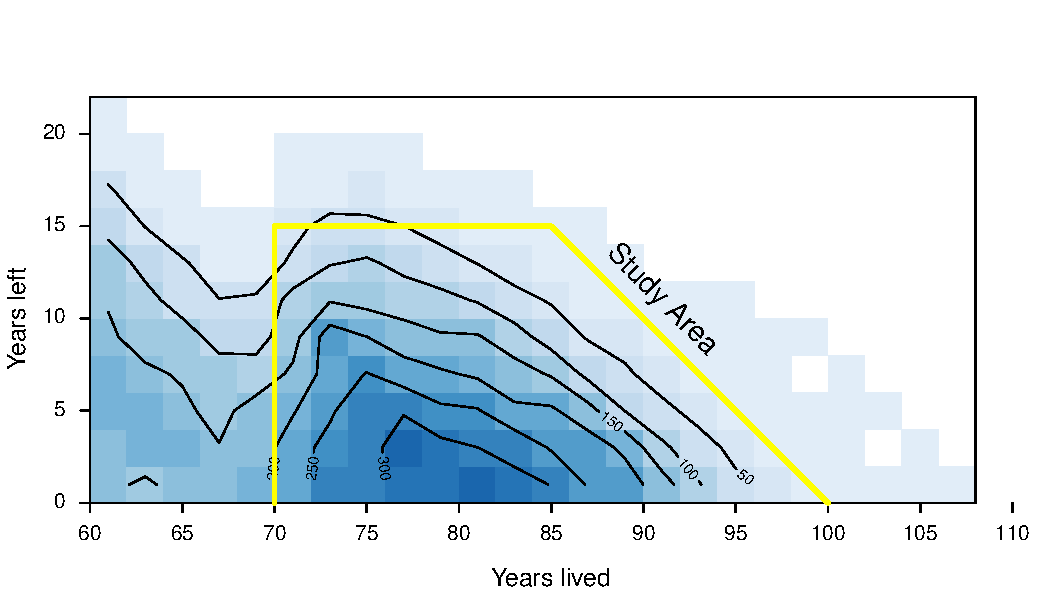
\includegraphics[scale=.7]{Figures/CaseCountMales.pdf}
\end{subfigure}
\\
\begin{subfigure}{\linewidth}
    \caption{Females}
   \vspace{-1em}
	\label{fig:FemalesCases}
    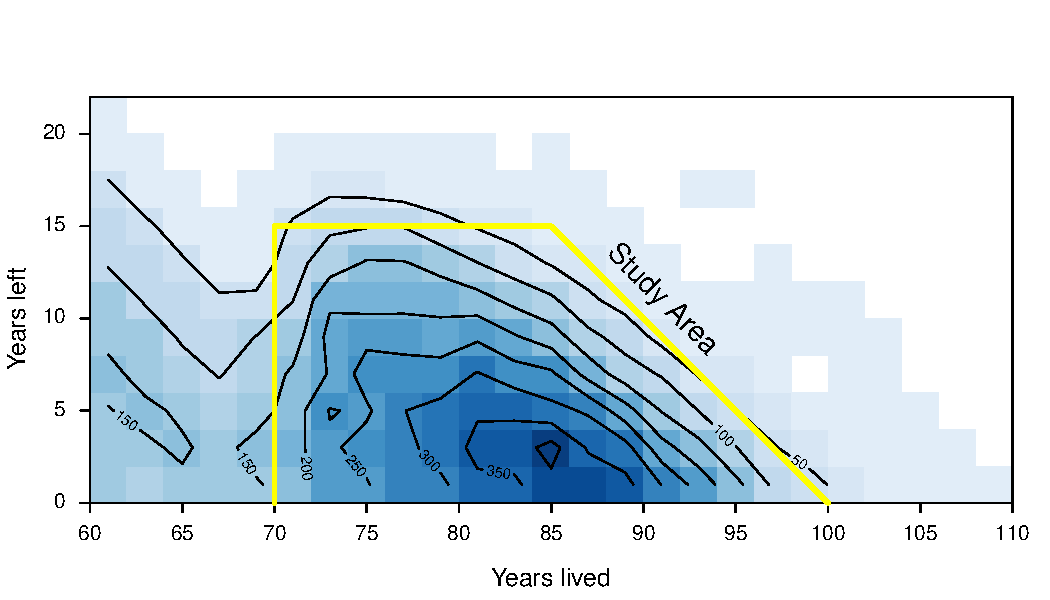
\includegraphics[scale=.7]{Figures/CaseCountFemales.pdf}
\end{subfigure}
\end{figure}

Note that Figure~\ref{fig:counts} resembles a Lexis surface in some ways, but it
is not organized by years or birth cohorts. Instead, years and birth cohorts in
the data are overlapped and treated as a single period and a single birth
cohort. We limit the study area to chronological ages 70 and higher, and
thanatological ages 15 and lower, and such that the sum of the two ages does not
exceed 100. These bounds allow for reasonably stable estimates of surfaces for
the studied characteristics. We cut off below chronological age 70 in order to
remove some patterns that appear to be due to retirement rather than some
senescent process, and also to avoid some potential compositional bias, as
these are the typical ages of recruitment for the HRS. Conceivably, the study
area could be expanded after the addition of future mortality follow-ups.

\subsection{Loess smoothing}
Direct tabulations of the weighted data are possible, and usually not too noisy,
but surface legibility is enhanced by estimating based on a loess-smoothed
surface. For each variable of interest, we convert values to a numeric scale.
For variables where a numeric scale is not the natural form of observation, we
describe the conversion protocol in an appendix\footnote{Variable appendix not
included in proposal.}. We then fit a two-dimensional loess model\footnote{We
fit using the \texttt{loess()} function in base \texttt{R}
\citep{cleveland1992local,Rcore2013} and its related prediction method. The
smoothing parameter, \texttt{spar}, is set to 0.5.} to the weighted
individual-level data for each sex separately, where the numeric characteristic value is the dependant variable and individual decimal values of thanatological and chronological age are the independent variables.
Weighting is then explicit by person-weights, and implicit by point density
within the surface. All individuals are included in the model fit, but point
predictions are calculated for a grid of single thanatological and chronological
ages within the study area outlined in Figure~\ref{fig:counts} and described in
the previous section. 

The model fit for each variable is used to produce a contour surface, which can
be interpreted visually. In most situations it is obvious to the eye whether a
variable operates over thanatological age or over chronological age, but there
are also some instances where both are at play, the pattern is evidently
distorted by underlying cohort heterogeneity, or where the relationship is
unclear.





\bibliographystyle{plainnat}
  \bibliography{references} 
  
\end{document}